\documentclass[twoside, UTF8]{EPURapport}
%\usepackage{listings}

%\renewcommand{\lstlistlistingname}{Liste des codes}
%\renewcommand{\lstlistingname}{Code}

%\addextratables{%
%	\lstlistoflistings
%}

%\swapAuthorsAndSupervisors


\usepackage{picinpar}
\graphicspath{Image}



\thedocument{Rapporte de stage de fin d'étude}{Développement d'un jeu sur iOS}{Développement d'un jeu sur iOS}

\grade{Département Informatique\\ 5\ieme{} année\\ 2011 - 2012}

\authors{%
	\category{Étudiant}{%
		\name{Fan ZHAO} \mail{zhao.fan@etu.univ-tours.fr}
	}
	\details{DI5 2010 - 2011}
}

\supervisors{%
	\category{Encadrant}{%
		\name{François Benaiteau} \mail{francois@chugulu.com}
	}
	\details{Chugulu Games}
}

\abstracts{Développement du jeu sur iOS. Ce rapport raconte mon stage de fin d'étude chez Chugulu Games. Y compris les concepts des développement du jeu, les techniques précisés etc.}
{iOS, jeux, développement}
{This repport is about the interneship at company Chugulu Games. The concepts about game develop, the process of game develop and the techniques used in game <<Playboy-Spots>>}
{iOS, game, develop}

\begin{document}

\chapter{Introduction} % (fold)

Le stage en 5ème année, qui est le stage de fin des études, pour pouvoir obtenir le diplôme, est obligatoire pour tous les étudiants au département informatique. La durée est au minimum 4 mois, au plus 5 mois, soit 20 semaines, pendant l’été 2011. 

Le stage de fin des études est très important pour un étudiant. Parce que la durée de ce stage est 4 mois, qui sont plus longs qu'avant. Aussi, après ce stage, nous allons diplômer. Nous devons chercher un boulot et commencer travailler. Nous serons plus étudiants. La durée de 4 mois nous permet d'avoir de la chance de participer dans un Éque. Travailler au dessus dans un grand projet. Pour cette durée, notre mission n’est plus les petites. Cela nous permet de toucher des mécanismes d'une entreprise, des contrôles des projets, des nouvelles techniques, des applications au niveau d'entreprise, des façons au niveau d'entreprise pour développer, etc. Aussi, nous pouvons rencontrer les gens, apprendre les nouvelles idées, etc. De l'autre coté, ce stage nous permet de savoir ce que nous en avons besoins, ce que nous aimer. Il est important puisqu’il y aura de la chance pour nous de continuer travaillé après stage. Même si nous n'aurons pas de chance de continuer, il peut nous donner quelques idées pour nous aider dans la future de recherches des travaux. Nous sommes bénéficié aussi à partir de ce stage, est que nous pouvons observer une vraie entreprise. Cela peut nous aider pour créer notre propre entreprise dans la future.

J’ai eu de la chance de trouver un stage dans l’entreprise Chugulu Games, qui est une entreprise à Tours, spécialisée dans le secteur des jeux. Mon stage a commencé du 23 mai, jusqu'au 30 septembre. Je travaille comme un développeur iOS. Ce stage est important pour moi, puisque travailler comme un développeur iOS est mon rêve. 

% chapter Introduction (end)

\chapter{Présentation} % (fold)

\section{Présentation de l'entreprise} % (fold)

\subsection{Chugulu Games} % (fold)

Chugulu Games est un studio de création spécialiste de la communication ludo-interactive et de l'advertainment. C'est concevoir et fabriquer des créations digitales (advergames,gaming banners, quiz interactifs, jeux multi-joueurs, serions games, social média applications) dont la dimension ludo-interactive, virale et communautaire est un accélérateur de notoriété et d'image de marque.

Voici le logo~\ref{fig:Image_Chugulu_Games1} de Chugulu Games.

Créée en 2006, Chugulu Games est une société spécialisée en advertainment. Nous concevons et fabriquons des créations digitales dont les dimensions ludique, virale et communautaire sont des accélérateurs de préférence de marque, de notoriété et de traffic.

Chugulu Games se concentre principalement sur 4 domaines principalement : Social Games, Jeux iPhone, Online Games et Unity 3D games. Comme le Figure~\ref{fig:Image_Chugulu_Games1} 


\begin{figure}[htbp]
	\centering
		
\includegraphics[width=6in]{Image/Chugulu-Games1.jpg}
	\caption{Logo de chugulu}
	\label{fig:Image_Chugulu_Games1}
\end{figure}

Principalement dire, Chugulu games a 2 type de jeux suivant le techniques utilisés. Un type est le jeu sur internet, souvent développé par flash. Ce type de jeu contient le jeu <BlindTest> qui a un site web de chugulu, souvent, les autres jeux sont basés sur des sites web sociale. Par exemple, facebook. L'autre type principal est le jeu sur iPhone. Chugulu games commence a développer des jeux de 3D basé sur Unity 3d. 

% subsubsection Chugulu Games (end)

\subsection{Equipe} % (fold)
\label{sub:subsection_name}

Chgulu games a 2 équipes. Une équipe est à paris, qui sont l'équipe principale, l'autre équipe est aux état-unis. Les 2 équipes sont présenté par le Figure~\ref{fig:Image_EquipeChugulu} suivant:

\begin{figure}[htbp]
	\centering
		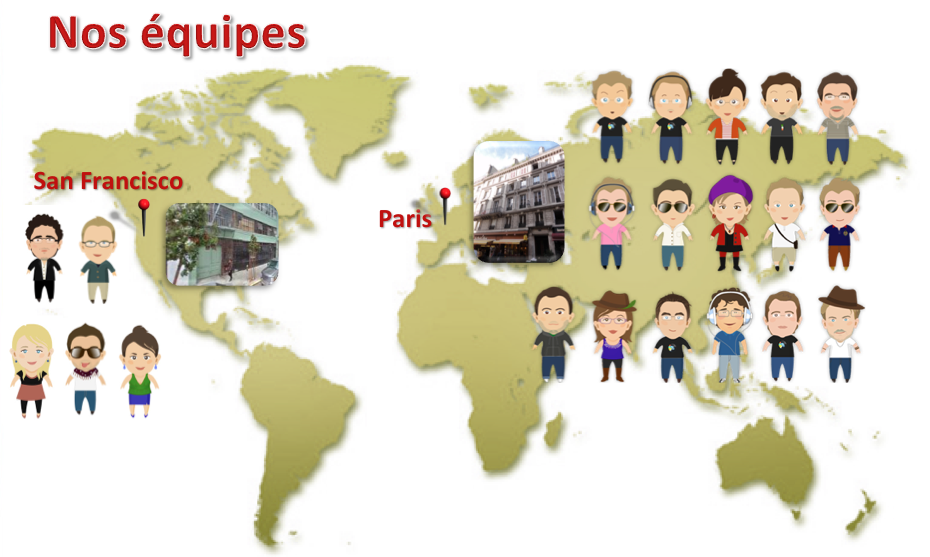
\includegraphics[width=6in]{Image/EquipeChugulu.png}
	\caption{L'équipe de chugulu games}
	\label{fig:Image_EquipeChugulu}
\end{figure}

Principalement dire, Chugulu games a 2 types de jeux suivant le technique utilisé. Un type est le jeu sur internet, souvent développé par flash. Ce type de jeu contient le jeu <BlindTest> qui a un site web de chugulu, souvent, les autres jeux sont basés sur des sites web sociaux. Par exemple, facebook. L'autre type principale est le jeux sur iPhone. Chugulu games commence a développer des jeux de 3D basé sur Unity 3d. 

% subsubsection Chugulu Games (end)


\subsection{Localisation} % (fold) \label{ssub:subsubsection_name}

Les jeux de chugulu games tous ont multi-language. Normalement, les jeux de chugulu games ont des versions d'anglais, version de français, version d'éspagnol. 

% subsubsection subsubsection_name (end)

\subsection{Références} % (fold) \label{ssub:références}

Chugulu games a travaillé avec plusieurs entreprises. Ses partenaires comportent des plus grandes entreprises françaises. Chugulu games a créé des jeux d'avertissements soie sur facebook, soie sur iPhone. Voici une liste des jeux.

Le Figure~\ref{fig:Image_chugulu_reference} liste quelques partenaires : 

% TODO chugulu references.


\begin{figure}[htbp]
	\centering
		
\includegraphics[width=6in]{Image/chugulu_reference.png}
	\caption{Les référence des produits de chugulu games}
	\label{fig:Image_chugulu_reference}
\end{figure}


\begin{itemize}
	\item LCL Open crémaillère \& 6:AM: Aménager entièrement son appart virtuel, et gagner réellement un an de loyer 
	\item Nokia Golden Goal \& Wunderman : Un advergame permettant de marquer plus de buts que l'équipe de France!
	\item Orange Snowballs \& Publicis Net : Un advergame pour i-Phone recréant une bataille de boules de neiges
	\item Air France \& La Chose : Un advergame s'inspirant du planisphère du magazine Air France
	\item Axe \& Buzzman : Un advergame prolongeant le film viral <<Canadairman>> pour la sortie d'AxeDry
	\item SFR \& EURO RSCG BETC 4D : Une réadaptation du Snake nokia 
	\item Renault \& Publicis Net : Contrer l'invasion de la dernière Scenic par des lapins vraiment très crétins
	\item Voyages SNCF \& Artdicted : Une narration ludo-pédagogique sur les gestes responsables du voyageur
	\item Prisma Press Group : Starbank, la bourse des people 
\end{itemize}

% subsubsection références (end)

\section{Advergame} % (fold) \label{sub:advergame}

\subsection{Définitions} % (fold) \label{ssub:définitions}

\begin{description}  \item[Advergame] : jeu développé pour le compte d’un annonceur.

\item[Casual gaming (ou jeu grand public)] : se dit des jeux vidéo s'adressant au plus grand nombre, femmes et seniors compris. Jeux présentant des gameplays simples et efficaces, compréhensibles en quelques secondes. Ex: PacMan, Tetris, AngryBirds, Doodle Jump, etc.

\item[Social gaming] : jeux grand public (ou pas) conçus pour être distribués sur les réseaux sociaux (facebook en particulier) dont les gameplay inclus des fonctionnalités sociales et virales. Ex : Farmville, Diner Dash, Mafiawars, etc.

\item[Serious game] : expérience ludique reprenant les codes du jeu vidéo, en vue de transmettre des acquis pédagogiques, responsables et/ou professionnalisants.

\item[Freemium] : modèle dans lequel la découverte du jeu est gratuite (free) et le gameplay propose des biens virtuels payants (premium).
\end{description}
Le définition sur le site Wikipédia est : L'advergame ou jeu vidéo publicitaire est un jeu vidéo qui cherche uniquement à promouvoir l'image d'une marque. Le mot advergame est un néologisme peu utilisé en France qui vient de la contraction de advertising (publicité) et de game (jeu). Un jeu vidéo publicitaire n'est pas à proprement parlé un serions game (jeu sérieux). Les serions games sont en effet des applications utilisant les technologies, techniques et usages du jeu vidéo, mais dans un but non ludique: apprendre à faire la cuisine, apprendre à faire quelque chose (médecine, etc.), etc.
Le jeu vidéo publicitaire est un jeu à part entière avec son côté ludique et justement non sérieux. C'est ce qui attire les annonceurs: l'univers jeu vidéo.

\subsection{Le marché de l'advergaming} % (fold) \label{ssub:le_marché_de_l_advergame}

Advergaming est un grand marché. Chiffre d’affaires mondial de 300 millions d’euros en 2010. Un taux de croissance annuel estimé à 47\% sur 2010 - 2015. Chiffre d’affaires 2015 estimé à 2 milliards d’euros. 40\% du top 100 des annonceurs français ont déjà eu recours à l’advergaming.

Au niveau de Fidélisation accrue des consommateurs, 61\% des joueurs déclarent avoir une meilleure opinion des produits présentés par un advergame. 50\% de la génération Y considèrent une marque plus crédible lorsqu'elle communique par le jeu.

Au niveau de Conversion prospect/client augmentée, 45\% des internautes satisfaits d’un advergame deviennent client de la marque.

% subsubsection le_marché_de_l_advergame (end)

% subsubsection définitions (end)

% subsection advergame (end) \subsection{Expérience technique} % (fold) \label{ssub:expérience_technique}

Chugulu game utilise plusieur techniques pour les jeux selon les besoins. Principalement, il existe 4 types de techniques. Ces 4 techniques sont les techniques moderne et populaire. 

\begin{description}  \item[Ruby on Rails] Rails est un framework open-source optimisé pour le bonheur des développeurs, engendrant une productivité accrue. Il combine simplicité, efficacité et modularité, ce qui nous permet de répondre facilement et rapidement aux besoins de nos clients. Utilisé par un nombre croissant de sites internationaux majeurs (Twitter, Yellow Pages, Github, Justin.tv, etc.), Ruby on Rails fait partie à ce jour des technologies web les plus dynamiques et les plus intéressantes de par sa communauté.

\item[Flash] est de très loin la solution la plus populaire pour diffuser du contenu interactif sur le web, car il est présent, selon Adobe, sur 99,5\% des ordinateurs connectés à Internet en Europe. La popularité de son clayer fait d’Adobe Flash un outil de développement et d’animation 2D très utilisé pour les jeux sur le web et pour les applications internet riches.

\item[L'iPhone] est aujourd'hui et depuis plusieurs années l'une des plateformes mobiles la plus plébiscitées par les usagers. Récemment l'iPad n'a fait que renforcer cette réalitée, c'est donc tout naturellement que Chugulu a consolidé son expérience dans cette technologie et plus largement dans les technologies mobiles.

\item[Unity 3D] Particulièrement concerné par les technologies les plus innovantes, Chugulu s’est familiarisé avec Unity3D, un moteur de rendu 3D destinée au développement de jeu vidéo jouables directement en page web, mais aussi sur iPhone, iPad et les smartphones Android. Son moteur graphique << next gen >> permet de créer des jeux proposant des rendus exceptionnels, disponibles sur un maximum de plateforme.
\end{description} % subsubsection expérience_technique (end)

\section{Introduciton au stage} % (fold)
Le mission de mon stage de fin d'études est développement et suivi des applications iPhone de la société. L'objective contient ces quatre points suivants : 


Mon stage à Chugulu Games peut être divisé en 2 parties. La première partie a duré 1 mois, commencé au début du stage. La première partie de stage s'est signifiée à travailler sur un projet qui s'appelle <<Télé7Jeux>>. La deuxième partie de stage a duré 3 mois, qui est la mission principale de mon stage. Dans la deuxième partie, j'ai travaillé sur un projet qui s'appelle <<Playboy-Spots>>.
\begin{itemize}  \item Savoir travailler en équipe.


\item Etre autonome sur une mission.

\item Respecter les consignes du lead développer iPhone  \item Faire preuve d'initiatives.
\end{itemize}


Mon stage à Chugulu Games peut être divisé en 2 parties. La première partie a duré 1 mois, commencé au début du stage. La première partie de stage s'est signifié à travailler sur un projet qui s'appelle <<Télé7Jeux>>. La deuxième partie de stage a duré 3 mois, qui est la mission principale de mon stage. Dans la deuxième partie, j'ai travaillé sur un projet qui s'appelle <<Playboy-Spots>>.


\subsection{Introductions au projet <<Télé7Jeux>>} % (fold) \label{ssub:introductions_au_projet_télé7jeux}

\begin{figure}[htbp]
	\centering
		
\includegraphics[height=3in]{Image/tele_7_jeux_logo_lien_logo.jpg}
	\caption{Le logo de télé7jeux sur iOS}
	\label{fig:Image_tele_7_jeux_logo_lien_logo}
\end{figure}


<<Télé7Jeux>> est un projet sur iPad. Il est annoncé par l'entreprise <<Lagardere>>. Ce jeu comporte tous les télé7jeux sur iPad, y compris <<Jeu de mémoire>>, <<Mot de réfléchir>>, <<Mot de croix>>, etc.. Ce projet est de mettre tous les jeux de télé7 sur iPad.
J'ai travaillé dans ce au début du stage. Le jour quand j'étais à Chugulu game, la game désigne a été déjà fini. Ce que j'ai fait est essayer de sortir une version prototype du jeu <<Jeu de mémoire>>. Le principe de prototype est d'essayer de développer une version qui fonctionne, sans graphiques, et donner une impression aux games désignées pour qu'eux, ils puissent savoir le résultat de leur designer. 


En fait, <<Télé7Jeux>> est un gros projet. Le prototype fait par moi est un des 5 jeux, qui est le plus simple, qui s'appelle <<Jeu de mémoire>>. Comme un débutant de développeur d'iOS, c'était super bien pour moi d'appliquer ce que j'ai appris, de comprendre les règles, les conventions de Chugulu Games. J'ai pris beaucoup de temps pour se familier avec les conventions des nommages, les règles des entreprises, les styles des codes, les façons des communications, les processus de travailler ensemble avec les membres dans l'équipe, etc. 

Cette partie de stage, même si qui n'a que duré un mois est hyper important pour moi.

% subsubsection introductions_au_projet_télé7jeux (end)

\subsection{Introduction au projet <<Playboy-Spots>>} % (fold) \label{ssub:introduction_au_projet_playboy_s}


\begin{figure}[htbp]
	\centering
		
\includegraphics[height=3in]{Image/logoPlayboy.png}
	\caption{Logo de <<Playboy-Spots>>}
	\label{fig:Image_logoPlayboy}
\end{figure}




Ce jeu signifie à créer un jeu sur iPhone, qui est un jeu comme les autres jeux du type 'différence'. De plus, ce jeu ressemble beaucoup à un des 5 jeux dans <<Télé7Jeux>>. Donc, nous avons mis beaucoup de temps pour discuter si nous pouvons utiliser les même, et les partagé entre les 2 projets. Après examiner au niveau du code, au niveau des concepts, au niveau de l'outil de version contrôle. Il nous semble impossible d'atteindre ce but. En fait, le gros problème est que, même si les 2 jeux ont les mêmes conceptions, ils ont quand même beaucoup de différences dans la base, qui nous bloque.

Ce projet va sortir 2 versions totalement sur App Store - une boutique d'Apple qui permettre aux entreprises de publier et vendre leurs applications. Les 2 types est la version Lite - qui est en fait la version gratuit, et la version Prenium - qui est en fait la version payante. Les différences entre ces deux versions peuvent être résumé comme :  \begin{itemize}  \item La version lite contient un nombre de photos fixé. 

\item La version Prenium contient une boutique qui fournit le possibilité d'acheter plusieurs packs dans le jeu. 
\end{itemize}
Ce modèle de business est utilisé souvent par les entreprises des jeux. 

Sauf la boutique, ce jeu comporte la synchronisation de serveur qui sert à télécharger les images, reporter les scores, reporter les stats des joueurs, recevoir les notifications, etc.. Un score board local basé sur la base des données locale et un score <<Game Center>> basé sur Apple.

Ce projet a commencé un mois après le début de mon stage. J'ai travaillé comme un membre dans l'équipe mobile. Le mois au début de ce projet, j'étais le seul développeur qui travaille sur ce projet. Pendant cette durée, j'essayer de sortir la structure des jeux, choisi les techniques utilisés, développés la première version, qui est en fait le prototype du jeu. A partir de deuxième mois, tous les autres développeurs ont joint dans ce projet, nous commençons ce projet.


Ce projet est le premier projet que je travaille dessus au début jusqu'à la fin. Dans ce rapport, je vais parler de ce projet.

% subsubsection introduction_au_projet_playboy_s (end)


% subsection Introduciton au stage (end)
% chapter Présentation (end)




\chapter{Techniques informatiques} % (fold)
\label{cha:techniques_informatiques}

Dans ce chapitre, je vais parle des outils et des techniques utilisés pendant ce stage. Ces outils contient les outils utilisé dans l'équipe pour le but de mieux communiquer et mieux collaborer. Il y a des outils utilisé pour développement, y compris l'IDE, les outils pour débug et amélioration etc. Sauf-ci, je vais quand même présenter les frameworks, conception utilisé pour ce projet.

\section{Outils de Collaboration} % (fold)
\label{sec:outils_de_collaboration}

Pendant ce stage, j'ai touché plusieurs techniques nouvelles, appris beaucoup des façons à développement. Sauf ci, j'ai appris beaucoup des outils de collaborations, et apprendre la façon de travaille en équipe. Dans ce section, je vais parler des outils de collaborations

\subsection{Producteev et Redmine} % (fold)
\label{ssub:producteev_et_redmine}

La raison de mettre les 2 outils ensemble est non seulement les 2 outils se ressemblent, mais aussi, ils sont les plus importantes. Au début de stage, dans un première temps, ce que j'ai touché est le Producteev. Producteev est utilisé par Chugulu Games pendant certaines années. Cet été, ils ont décidé de changé à utiliser un autre outil qui s'appelle Redmine. 

\subsubsection{Producteev} % (fold)
\label{ssub:producteev}

% TODO Add the logo Producteev:

Producteev est un gestionnaire de tâches à la fois B2B et B2C dont l’ADN est collaboratif. D’une utilisation personnelle à un nombre de connectés illimités en entreprise, la solution fonctionne online et offline en interface avec les comptes e-mail, Facebook ou Google Calendar entre autres dans des versions web et mobiles. Il a ces fonctionnalités :
\begin{description}
	\item[Gestion de plusieurs équipes] Gérer plusieurs équipes grâce à Producteev en utilisant les fonctionnalités simples intégrées. Inviter les membres des équipes, ajustez les paramètres de confidentialité et bien plus encore pour votre liste de tâches.
	\item[Filtres et rapports] Générer facilement des rapports sur le projet et sur l'activité d'équipe. Par exemple, recevoir toutes les semaines un email d'aperçu des avancées d'équipe.
	\item[Emails récapitulatifs] Recevez chaque jour le rapport journalier/hebdomadaire, pour avoir un aperçu de l'équipe.
	\item[Tâches prioritaires]  L'algorithme utilisé pour la gestion des tâches prioritaires trie automatiquement les tâches et  suggère à faire ensuite
	\item[Synchroniser vos tâches avec Google Agenda] Synchronisez Producteev avec Google Agenda ou placer-y simplement une tâche à la fois. 
\end{description}

Sauf ces fonctionnalité, producteev est possible de synchroniser avec ses logiciel client sous Mac ou iPhone, avec Google. Et, il est possible de se communiquer en utilisant les mails. Envoyer et recevoir les nouvelles par les mails. 

% subsubsection producteev (end)

\subsubsection{Redmine} % (fold)
\label{ssub:redmine}

% TODO add the logo

Redmine est une application web Open Source de gestion complète de projet en mode web, développé en Ruby sur la base du framework Ruby on Rails.
Il a été créé par Jean-Philippe Lang. D'autres développeurs venant de la communauté des utilisateurs de Redmine contribuent depuis au projet. Il utilise la syntaxe Textile pour ses pages de wiki et de nombreux autres emplacements où l'utilisateur peut entrer du texte : 
\begin{itemize}
	\item descriptif de bogue ou de demande, ainsi que les commentaires associés
	\item forums
	\item nouvelles
	\item description
\end{itemize}

La fonctionnalité de Redmine comporte la liste suivante:
\begin{itemize}
	\item gestion multi-projets
	\item gestion fine des droits utilisateurs définis par des rôles
	\item gestion de groupes d'utilisateurs
	\item rapports de bogues (bugs), demandes d'évolutions
	\item Wiki multi-projets
	\item forums multi-projets
	\item news accessibles par RSS / ATOM
	\item notifications par courriel (mail)
	\item gestion de feuilles de route, GANTT, calendrier
	\item historique
	\item intégration avec divers suivis de versions : SVN, CVS, Mercurial, Git, Bazaar & Darcs
	\item identification possible via LDAP
	\item multilingue (25 langues disponibles pour la 0.7.0)
	\item support de plusieurs bases de données : MySQL, PostgreSQL ou SQLite
\end{itemize}

Par rapport au Producteev, redmine a des avantages evident. La plus importante est que redmine est gratuit. Il est possible d'installer redmine dans le site web interne d'entreprise. Il a un système de notification mieux que producteev. Redmine supporte beaucoup de personnalisation. Il permet de personnalisé les couleur, les interfaces etc. De plus, redmine supporte 30+ de language. 

Pendant ce stage à chugulu, nous avons utilisé beaucoup cet outil pour se communiquer, mettre à jours nos statues. Il est aussi facile pour le chef de projet, pour mon encadrant de reporter les nouvelles issus, de contrôle les progrès des tâches assigné à chaque développeur. L'interface de redmine est beaucoup mieux par rapport à l'interface de producteev. Sur redmine, nous pouvons mettre à jours nos tâches et nos statues simplement par cliquer à droit sur la souris. 

Un autre avantage important est qu'il peut être installé à interne de l'entreprise. C'est beaucoup mieux par rapport à un site web comme Producteev. Non seulement la niveau de sécurité, mais aussi que on peut maintenir nous même. Si un jour, Producteev est disparu, nous allons perdre tous nos informations.

% subsubsection redmine (end)

% subsubsection producteev_et_redmine (end)

\subsection{Git \& Github} % (fold)

\subsubsection{Git} % (fold)

% TODO add git

Git est un logiciel de gestion de versions décentralisée. C'est un logiciel libre créé par Linus Torvalds, le créateur du noyau Linux, et distribué sous la GNU GPL version 2. Il est crée par Linus Torvalds, qui est aussi le créateur de Linux. Git ne repose pas sur un serveur centralisé. C'est un outil bas niveau, qui se veut simple et très performant, dont la principale tâche est de gérer l'évolution du contenu d'une arborescence. Chaque répertoire git contient une base des données local, y contient toutes les fichiers, les commits, les traces, les branches etc. Il est encore un avantage par rapport aux autre logiciel version contrôle comme SVN, c'est que git nous permet de choisi un ou plusieurs fichier. 

Git possède deux structures de données : une base d'objets et un cache de répertoires. Il existe quatre types d'objets :

\begin{itemize}
	\item l'objet blob, qui représente le contenu d'un fichier (l'origine de cette dénomination est probablement à chercher dans les Binary Large OBjects des bases de données).
	\item l'objet tree ("arbre" en anglais), qui est une liste d'objets de type blobs et des informations associées à chaque blob, tel que le nom du fichier et les permissions. Cet objet décrit l'arborescence des sources à un temps donné.
	\item l'objet commit, qui donne accès à l'historique d'une arborescence de source. Il contient un message de log, un objet arbre et pointe vers un ou plusieurs objets commit parents.
	\item l'objet tag qui est une manière de représenter un commit spécifique. Il est en général utilisé pour marquer certains commits, par exemple par un numéro ou un nom de version (2.1 ou bien Hardy Heron).
\end{itemize}

La base des objets peut contenir n'importe quel type d'objets. Une couche intermédiaire, utilisant des index (les sommes de contrôle), établit un lien entre les objets de la base et l'arborescence des fichiers.
Chaque objet est identifié par une somme de contrôle SHA-1 de son contenu. Git calcule la somme de contrôle et utilise cette valeur pour déterminer le nom de fichier de l'objet. L'objet est placé dans un répertoire dont le nom correspond aux deux premières lettres de la somme de contrôle. Le reste de la somme de contrôle constitue alors le nom du fichier pour cet objet.

Git enregistre chaque révision dans un fichier en tant qu'objet blob unique. Les relations entre les objets blobs sont déterminées en examinant les objets commit. En général, les objets blobs sont stockés dans leur intégralité en utilisant la compression de la zlib. Ce principe peut rapidement consommer une grande quantité de place disque ; de ce fait, les objets peuvent être combinés dans des archives, qui utilisent la compression différentielle (c'est-à-dire que les blobs sont enregistrés sous la forme de différences par rapport aux autres blobs).
% subsubsection Git (end)

\subsubsection{Github} % (fold)

% TODO add logo github

GitHub est un service web d'hébergement et de gestion de développement de logiciels, utilisant le programme Git. Ce site est développé en Ruby on Rails. GitHub propose des comptes professionnels payants, ainsi que des comptes gratuits pour les projets open source. Il est le meilleur site web du monde pour utiliser git. Github supporte la collaboration. Il supporte le fonction de folk. Nous pouvons faire une copie de n'importe quel projet qui nous intéresse. Github supporte plusieurs type de management. Par défaut, nous pouvons avoir une répertoire gratuits, mais tous nos fichiers sont publié. Github fournit quelque options pour les utilisateurs d'entreprise. Par exemple, nous pouvons payer 7 dollar par mois, et obtenons 5 repositoir avec 1 collaborateur, qui peut avoir 0.6GB d'espace. 

Github travaille mieux par rapport aux serveur de svn chez Chugulu Game. Chugulu games a commencé à utiliser git & github cet été. Il devient mieux par rapport avant.
% subsubsection Github (end)

% subsection Git \& Github (end)

\subsection{XMind} % (fold)

% TODO add logo XMind.

XMind est un outil très pratique. Chugulu game utilise cet outil beaucoup pour organiser les idées, présenter les schémas. 

XMind est un logiciel Open Source, pour brainstorming. Il a deux version, une version gratuit et une version plus puissante mais payante. XMind est basé sur Eclipse, qui fournit l'assistance aux utilisateurs de trouver ses idées, organiser différente type des schémas, partager avec leur collaborateurs. Il supporte Mind Map, Ishikawa diagrams (fishbone diagrams ou cause-and-effect diagrams), tree diagrams, organization charts, et spreadsheets. Il est possible de l'utiliser pour manager les savoir-faire, les notes des conférences, et GTD. 

La version payante supporte exporter les mind map en format Microsoft Word, Power point, PDF etc.

Pendant ce stage, j'ai utilisé XMind pour organiser mes idées, construire les schéma nécessaire, et les a inséré dans les documents internes. En utilisant XMind, j'ai gagné beaucoup de temps. C'est aussi important et facile pour moi de mieux présenter mes idées.

% subsection XMind (end)
% section outils_de_collaboration (end)

\section{Outils de Développement} % (fold)
\label{sec:outils_de_développement}

\subsection{XCode} % (fold)
\label{sub:xcode}

% TODO add logo xcode

XCode est un environnement de développement pour MacOS. Il est crée par l'entreprise Apple, et utilisé seulement sous MacOX. XCode est un IDE très puissante. Il comporte presque toute les caractéristiques commune des IDE, sauf ci, il supporte des techniques spécial pour améliorer la productivité sous MacOS. XCode supporte plusieurs langage, y compris C, C++, Objective C, PHP, Ruby, etc.. XCode fournit une interface unifié, respecter le standard d'interface de MacOS. Il est très facile à apprendre pour un utilisateur de MacOS. Surtout XCode 4, il fournit une interface comme iTunes. Fourni avec toute une suite logicielle (graphiques, audio, etc.) pour développeurs et programmeurs, il permet de créer des logiciels utilisant toutes les fonctionnalités, la puissance et la stabilité de Mac OS X et d'UNIX. Par rapport aux Visual Studio de Microsoft, cet IDE est gratuit.

Maintenant, la nouvelle version est XCode 4.1. 

Le raison pour choisir XCode comme l'IDE principale est évident. Parce que, il est la seule choix pour développer l'application sur iOS. Il supporte les plus de fonctionnalité, les outils pour développer. Il est aussi désigné et amélioré spécialement pour iOS développé. Il n'as pas de raison pour ne pas utiliser ce produit.

% subsection xcode (end)

\subsection{Instruments} % (fold)
\label{sub:instrument}

% TODO add log instruments

Instruments est un logiciel crée par Apple. Il est un outil hyper fort. Instrument est un logiciel pour développeur de tracer et profiling le projet MacOS et iOS dynamiquement. Il est très pratique pour débugger, résoudre le performance d'application. Il est aussi très utile pour améliorer le performance. Pendant ce stage, j'ai utilisé cet outil pour améliorer la performance de <<Playboy-Spot>>. 
Voici une capture de l'écran quand j'ai fait tracer tous les threads pendant l'exécution. 

% TODO add instrument capture d'écran
% subsection instrument (end)

% section outils_de_développement (end)

\section{Technique utilisé} % (fold)
\label{sec:technique_utilisé}

% section technique_utilisé (end)


% chapter techniques_informatiques (end)

\chapter{Développement d'un jeu} % (fold)
\label{cha:développement_d_un_jeu}

Dans ce chapitre, je vais parler du développement du jeu <<Playboy-spots>>. <<Playboy-spots>> est le premier jeu que j'ai participé dans ma vie. Au début jusqu'au produit finale. Pendant ces processus de développement, j'ai appris beaucoup de chose, concept etc. Non seulement que j'ai appris beaucoup, mais aussi, grâce à ce projet, j'ai commencé à réfléchir beaucoup, comparer les techniques utilisés, résumer les points négative et positive. Ces expérience vont m'aider beaucoup dans les projets futurs. Dans n'importe quelle entreprise.

\section{Processus} % (fold)
\label{sec:processus}

Un jeu est un logiciel spéciale. Au niveau de ressource, un jeu est plus difficile à développer par rapport aux logiciel. Parce que un jeu demande beaucoup de ressource par rapport aux logiciels. Je vais le parler dans section suivant. Au niveau de processus de développement. Un jeu est plus simple par rapport aux logiciel. Ici, je vais parler le processus de développement d'un jeu en général et en comparant avec le processus réel chez chugulu games. surtout, il faut savoir, ici, le processus est utilisé par les petites équipes. Pour les grandes entreprises comme <<EA>>, ils ont un autre processus plus complet, plus systématiques, mais va durer plus long, et leurs processus est utilisé pour créer des jeux gros. Pour chugulu games et billions des studio comme chugulu games, leurs caractéristiques commune sont petite, bouger simple, réactiver rapide, développer rapide. 

\subsection{Processus Général} % (fold)
\label{sub:processus_général}

En générale, au niveau de programmation, le processus général n'est pas très loin que la processus classique d'un logiciel. Le processus peut être décomposé en plusieurs étape, qui sont présentés dans le schéma comme figure~\ref{fig:}.

% TODO add schéma générale

Dans ce figure, on peut voir, généralement, un développement du jeu peut être divisé en les étapes suivantes :

\subsubsection{Collect ideas} % (fold)

Développer un jeu peut avoir plusieurs raison. Peut être, nous avons trouvé des idées très intéressantes. Peut-être, nous avons trouvé que dans la marché du jeu, il manque ce genre de jeu, donc, le jeu ce que nous faisons va être réussis dans la futur. Peut-être, nous allons regarder un jeu qui est déjà réussis, qui a vendu billiard euros, et nous décidons de juste créer un jeu qui ressemble, mais en même temps, plus <<Intelligent>>. Peut-être, peut-être... Nous avons mille d'excuse pour créer un jeu. Pareil, selon les type de jeu, selon l'entreprise, nous pouvons avoir plusieurs processus totalement différent pour créer un jeu. 

Mais, dans toutes les processus différente, il existe un étape commune, essentiel et importante. C'est l'étape de collection des idées. 

Cet étape signifie à définir un principe du jeu en générale. Après cet étape, nous devons être sure que, notre jeu doit afficher quoi, comment jouer notre jeu. Donc, dans cet étape, ce que nous nous discutons est la chose la plus importante. 

Un autre point à savoir, c'est que, dans cet étape, souvent, nous savons pas les interfaces doivent afficher comment. Dans cet étape, souvent, une entreprise va organiser plusieurs réunions.

Dans le jeu de <<Playboy-Spots>>, dans cet étape, nous avons réussi a déterminer la coeur du jeu. Par exemple, nous savons que, nous avons plusieurs pack, chaque pack contient certaines photos. Nous savons que, sur chaque photo, il y aura certaine différences à trouver. Le nombre des différence n'est pas fixé, peut être 5, peut être 4. Nous savons que, nous avons 3 mode de jeu, sur chaque mode, le jeu va être joué différemment etc..

% subsubsection Collect ideas (end)

\subsubsection{Game Design} % (fold)

Dans cet étape, les game désigners vont commencer désigner le jeu. Concernant n'importe quel élément dans le jeu. Game désigners vont essayer de déterminer toutes les interfaces, les mécanismes (par exemple, les mécanisme de scoring, etc.) Les désigners vont essayer de sortir toutes les mock-up sur toutes les interfaces. 

En fait, cet étape est un début d'un cycle. Ce cycle commence par game désign, ensuite, les développeurs vont essayer de sortir une prototype, et à la fin, les développeurs vont montrer le prototype aux game désigners pour qu'ils puissent regarder ce qui donne, puissent savoir s'il y a des problème au niveau de conception, mécanisme, etc. Ce cycle peut durer longtemps, puisque, un jeu n'égale pas à un logiciel. Nous ne savons pas si nos désignes sont bonne ou pas, intéressantes ou pas. Donc il est essentiel de regarder notre idée devient réel, et jouer en réel. S'il y a des choses qui ne marchent pas, nous pouvons avoir de la chance de corriger avant commencer à programmer.

Normalement, après cet étape, nous devons être capable de sortie un cahier qui décrit toutes nos designs pour que nous puissions commencer développer.

% subsubsection Game Design (end) 

\subsubsection{Prototype} % (fold)

Dans les petite entreprise, ou les petits studios, cet étape est important. Souvent, dans ce cas, nous n'avons pas beaucoup de développeur, ni beaucoup de temps. Souvent, les jeux que nous allons développé ne sont pas gros. Ils sont les petite jeux. Il est possible de créer les prototypes dans ces cas. 

Un prototype est défini pas wikipédia comme suivante : Un prototype désigne le premier, ou l'un des premiers exemplaires d'un produit industriel (voiture, avion…). Cet exemplaire permet de faire des tests afin de valider les choix de conception de l'ensemble. Le prototype précède les exemplaires de pré-série. 

Dans le développement du jeu, notre prototype va déterminer le structure du jeu, les fonctionnalités générales dans le futur. 

% subsubsection Prototype (end)

\subsubsection{Work} % (fold)

Quand nous allons dans cette étape, nous somme sure que toutes les désigns sont déjà fait, validé par game désigner. Il n'existe pas grand problème dans prototype. Nous avons bien déterminer les éléments du jeu. Donc, nous pouvons commencer développer. 

Cette étape va duré longtemps, tous membres dans l'équipe vont rejoindre dans ce projet. En même temps, toutes les autre équipe vont commencer à travailler, par exemple l'équipe de graphiste, l'équipe de musique etc.. 

En fait, cette étape peut être divisé en plusieurs sous étapes. Prendre le programmation comme exemple, nous pouvons décomposé en plusieurs comme <<Faire la cahier de charge>>, <<Construire la structure général>>, etc..

% subsubsection Work (end)

\subsubsection{Beta} % (fold)

L'étape suivant est l'étape de Beta. Dans cette étape, normalement, nous avons bien développé notre jeu. Même s'il y a beaucoup des bugs, des erreurs, des fonctionnalités qui ne marchent pas. Le but de cette étape est de tester s'il y a gros problème à corriger. Non seulement les bugs qui font crasher le jeu, mais aussi les designes qui n'a pas l'air bien et utile. Dans ces 2 cas, il faut que nous collectons tous des informations nécessaires, trouvons des solutions, et donner aux développeurs ou désigners de soit corriger les bugs soit redésigner. 

Cette étape peut se répète plusieurs fois. En fait, aucun jeu peut être publié directement après développement. Ce n'est pas du tout possible. Il est normale d'avoir plain de bugs dans un jeu. Le jeu le plus gros 



% subsubsection Beta (end)



% subsection processus_général (end)

% section processus (end)

% chapter développement_d_un_jeu (end)

\chapter{Conclusion}

Ce stage est une expérience très important pour moi.C’est vraiment une expérience importante et magnifique pour moi de travailler à Chugulu. Grâce à vous, j’ai trouvé mon métier de prédilection.

J’ai développé le moteur de jeu du <<Playboy-spots>>. Dans le futur, il y aura certains projets qui sont basés sur ce moteur. S'il y aura des projets simulaire, je peux travailler dessus directement. Je n’ai pas besoins de relire le code, de familier avec les frameworks utilisées. 

Pendant ce stage, j’ai appris beaucoup en suivant les instructions de mon encadrant. Non seulement les techniques utilisées, les outils de collaborations, mais aussi les façons de communications, les façons de travailler dans l’équipe.  Les techniques ne sont pas difficiles à apprendre. L’équipe chugulu est une grande famille, ils sont tous très gentil pour moi un étranger. Grace à eux, j’ai trouvé mon métier de prédilection. J’aime travailler dans l’industrie du jeu. Et j’ai de la chance de travailler dans une entreprise qui est le leader en France. Et dans la futur, je peux touché beaucoup de techniques nouvelles, avoir des expériences de jeux.



\annexes

Ici, je vais ajouter quelque capture du jeu <<Playboy-Spots>>.
\begin{figure}[htbp]
	\centering
		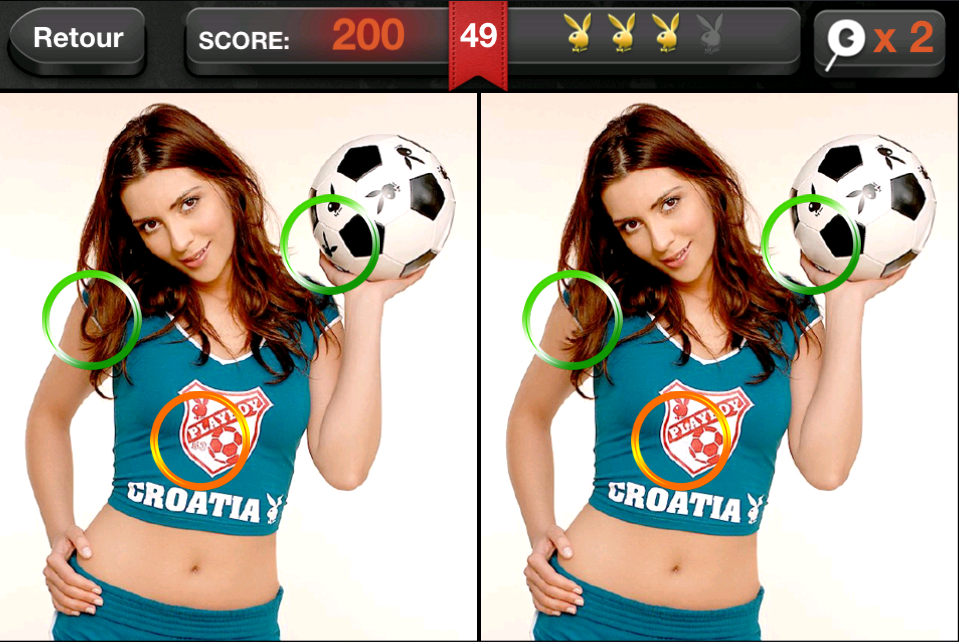
\includegraphics[height=3in]{Image/Capture1.png}
	\caption{Le jeu}
	\label{fig:Image_Capture1}
\end{figure}
\begin{figure}[htbp]
	\centering
		
\includegraphics[height=3in]{Image/Capture2.png}
	\caption{Capture de la boutique}
	\label{fig:Image_Capture2}
\end{figure}
\begin{figure}[htbp]
	\centering
		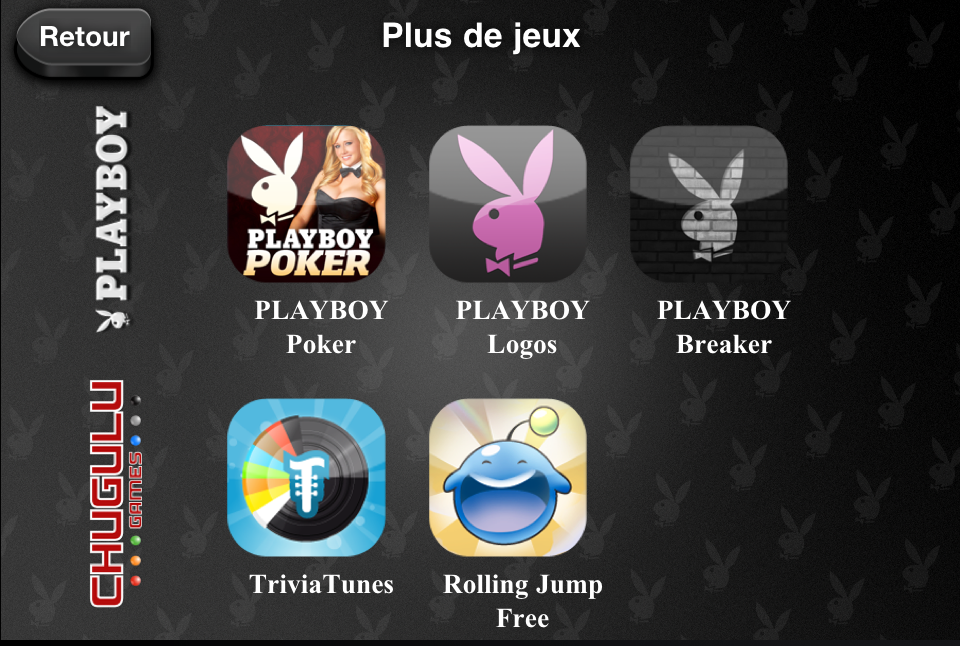
\includegraphics[height=3in]{Image/Capture3.png}
	\caption{More games}
	\label{fig:Image_Capture3}
\end{figure}
\begin{figure}[htbp]
	\centering
		
\includegraphics[height=3in]{Image/Capture4.png}
	\caption{Crédit}
	\label{fig:Image_Capture4}
\end{figure}


\end{document}

